\documentclass{article}
\usepackage[utf8]{inputenc}
\usepackage{amsmath}
\usepackage{graphicx}
\usepackage{tabularx}
\usepackage{xcolor}
\usepackage{tabularray}
\usepackage{float}
\usepackage{bm}
\usepackage[colorlinks]{hyperref}
\usepackage[normalem]{ulem}
\usepackage[affil-it]{authblk}
\setlength{\parindent}{0pt}
\usepackage{caption}
\captionsetup[table]{position=bottom} 
%\usepackage{draftwatermark}
%\SetWatermarkText{Draft}
%\SetWatermarkScale{4}
%\SetWatermarkColor[gray]{0.97}

\usepackage{titlesec}

\setcounter{secnumdepth}{4}

\titleformat{\paragraph}
{\normalfont\normalsize\bfseries}{\theparagraph}{1em}{}
\titlespacing*{\paragraph}
{0pt}{3.25ex plus 1ex minus .2ex}{1.5ex plus .2ex}

\title{Peace Agreement Signatories Analysis}
\author{Roy Gardner}

\begin{document}

\newcolumntype{R}{>{\raggedleft\arraybackslash}X}

\maketitle

\tableofcontents
\newpage

\section{Motivation}

To provide a useful abstraction from which to explore the agreements-actors signatory dataset.

\section{Agreement-Actor Matrix}

A binary-valued matrix is a matrix containing values from $\{0,1\}$ that can be used to represent binary relations between members of a pair of sets. For example, whether or not an actor is a signatory to a peace agreement.\newline

For any binary-valued agreement-actor matrix there is an indexed set of agreements 

\begin{equation}
A=\{a_1,a_2,…,a_M\}
\end{equation}

where $M$ is the total number of agreements, i.e., $M=|A|$.\newline

There is an indexed set of signatory actors

\begin{equation}
S=\{s_1,s_2,…,s_N\} 
\end{equation}

where $N$ is the total number of actors, i.e., $N=|S|$.\newline

Each agreement $a_i$ has a set of signatories 

\begin{equation}
S_{i}\subset S
\end{equation}

Each actor $s_j$ has a set of agreements to which they are a signatory.

\begin{equation}
A_{j}\subset A
\end{equation}

A binary-valued matrix $\bm{U}$ is generated with agreements in rows and actors in columns. Cells values are given by:

\begin{equation}
u_{ij} =
\begin{cases}
0& if \ s_j \notin S_{i}\\
1 & if \ s_j \in S_{i}
\end{cases}
\end{equation}


\subsection{Graphs}

A binary-valued matrix describes an undirected bipartite graph where members of one set are connected to members of the other set, but where within-set connections do not exist. \newline

A graph of the agreement-actor matrix of the Bosnia peace process is show in Figure 1 of Appendix A.1.\newline

A graph can be queried using depth-first search to show only the network of relations between a combination of selected actors and/or agreements. A search can be run against the binary matrix or against the graph if search is supported by the graph package. \newline

A graph of a search against the Bosnia peace process is show in Figure 2 of Appendix A.2.\newline

\section{Agreement-Actor Co-occurrence Matrices}

\subsection{Actor co-occurrence matrix}

The actor co-occurrence matrices provides the number of agreements to which a pair of actors are co-signatories.\newline

The actor co-occurrence matrix is given by

\begin{equation}
\bm{V = U^TU}
\end{equation}

where $\bm{V}$ is a symmetric matrix with the $N$ actors of $\bm{U}$ in both rows and columns. The diagonal of $\bm{V}$ provides the columns marginal of $\bm{U}$.\newline

A cell value contains the number of agreements to which a pair of actors are both signatories:

\begin{equation}
v_{ij} =  |(A_{i} \cap A_{j}) | 
\end{equation}

i.e., the cardinality of the intersection of the agreement sets of the row actor $s_i$ and the column actor $s_j$. \\

The set of indices $I_{ij}$ of the agreements in a cell $v_{ij}$ are the indices of non-zero values in the result of a bitwise AND between the $i^{th}$ and $j^{th}$ rows of $\bm{U^T}$:

\begin{equation}
\bm{x} = \bm{(U^T)}_i \land \bm{(U^T)} _j
\end{equation}

\begin{equation}
n =
\begin{cases}
\in I_{ij} & if \  \bm{x}_n = 1\\
\notin I_{ij} & f \  \bm{x}_n = 0
\end{cases}
\end{equation}

\subsection{Agreement co-occurrence matrix}

The agreement co-occurrence matrices provides the number of actors that are co-signatories to a pair of agreements.\newline

The agreement co-occurrence matrix is given by

\begin{equation}
\bm{W= UU^T}
\end{equation}

where $\bm{W}$ is a symmetric matrix with the $M$ agreements of $\bm{U}$ in rows and columns. The diagonal of $\bm{W}$ provides the rows marginal of $\bm{U}$.\newline

A cell value contains the number of actors that are co-signatories to a pair of agreements:

\begin{equation}
w_{ij} =  |(S_{i} \cap S_{j}) | 
\end{equation}

i.e., the cardinality of the intersection of the actor sets of the row agreement $a_i$ and the column agreement $a_j$. \\

The set of indices $I_{ij}$ of the actors in a cell $w_{ij}$ are the indices of non-zero values in the result of a bitwise AND between the $i^{th}$ and $j^{th}$ rows of $\bm{U}$:

\begin{equation}
\bm{x} = \bm{(U)}_i \land \bm{(U)} _j
\end{equation}

\begin{equation}
n =
\begin{cases}
\in I_{ij} & if \  \bm{x}_n = 1\\
\notin I_{ij} & f \  \bm{x}_n = 0
\end{cases}
\end{equation}

\subsection{Graphs}

An actor co-occurrence matrix can be represented as a graph where vertices are actors connected by edges with a weight given by the number of agreements to which the actors are co-signatories.  The graph can be used to explore actor-actor relationships within a peace process including the existence of disjoint subgraphs and triadic closures. See Figure 3 in Appendix A.3 for an example from the Bosnia peace process. \newline


\section{Process-Actor Matrix}

The methods described above can be applied to peace process-actor matrices.\newline

There is an indexed set of processes 

\begin{equation}
P=\{p_1,p_2,…,p_M\}
\end{equation}

where $M$ is the total number of peace processes, i.e., $M=|P|$.\newline

There is an indexed set of signatory actors

\begin{equation}
S=\{s_1,s_2,…,s_N\} 
\end{equation}

where $N$ is the total number of actors, i.e., $N=|S|$.\newline

Each process $p_i$ has a set of signatories 

\begin{equation}
S_{i}\subset S
\end{equation}

Each actor $s_j$ has a set of processes in which they are a signatory to at least one agreement.

\begin{equation}
P_{j}\subset P
\end{equation}

A binary-valued matrix $\bm{C}$ is generated with agreements in rows and actors in columns. Cells values are given by:

\begin{equation}
c_{ij} =
\begin{cases}
0& if \ s_j \notin S_{i}\\
1 & if \ s_j \in S_{i}
\end{cases}
\end{equation}

\appendix

\section{Visualisations}

\subsection{Graph of agreement-actor matrix}

\begin{figure}[H]
\begin{center}
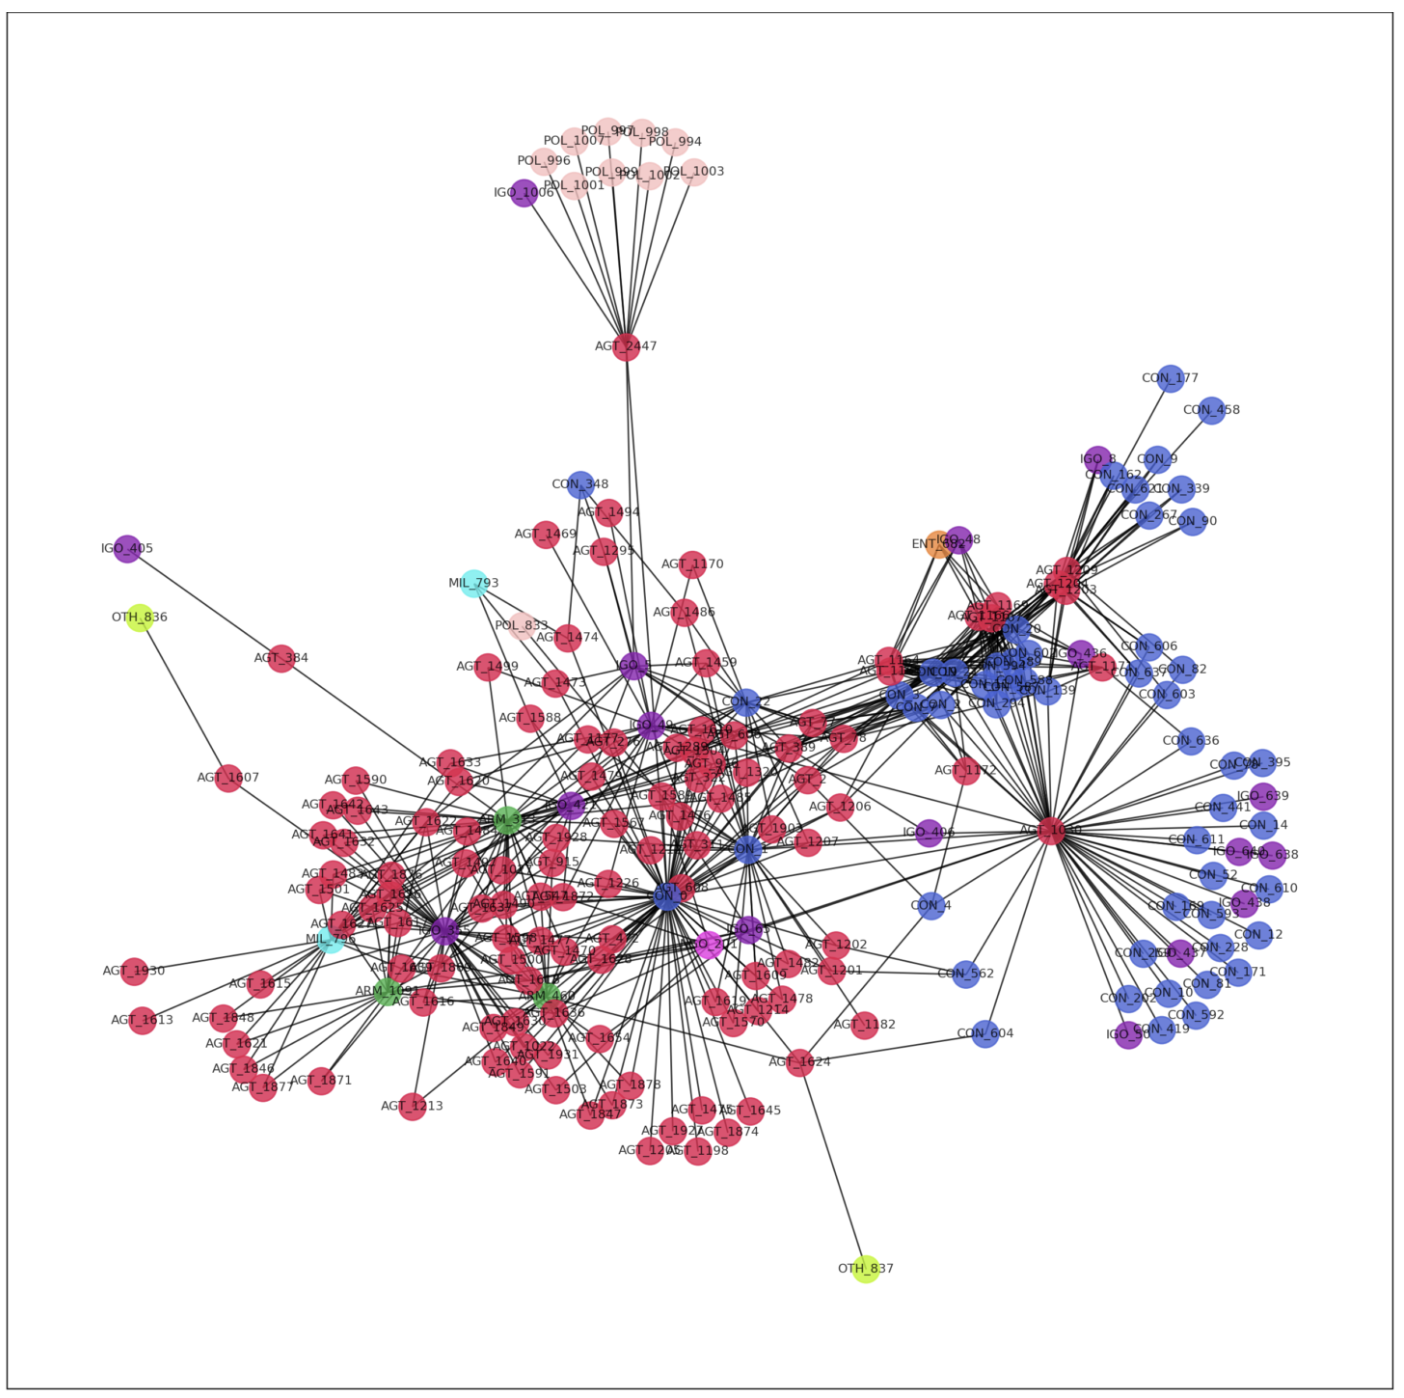
\includegraphics[scale=0.50]{./assets/bosnia_process.png}
\end{center}
\caption{A graph of the binary-valued agreement-actor matrix for the Bosnia peace process. Vertices in red are agreements. Actors are colour coded by type, for example, countries in blue.}
\end{figure}

\subsection{Graph of agreement-actor matrix search results}

\begin{figure}[H]
\begin{center}
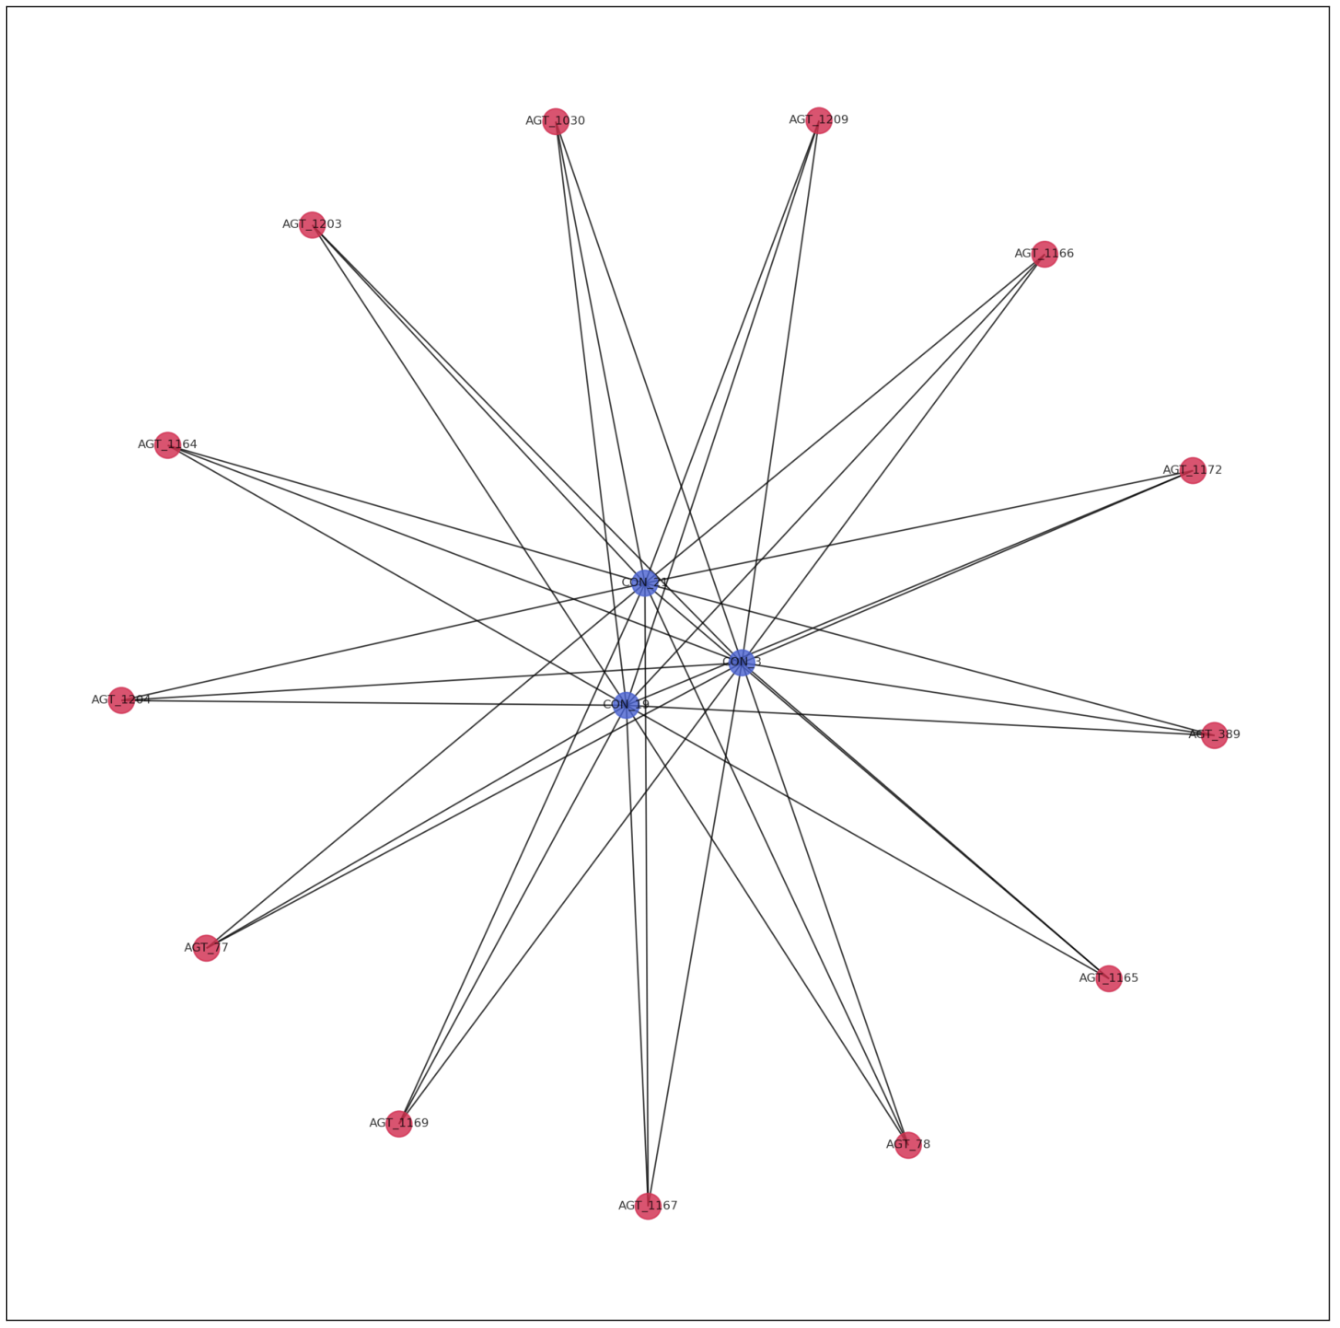
\includegraphics[scale=0.50]{./assets/bosnia_query.png}
\end{center}
\caption{A graph of the results of a depth-first search for the actors Russia, UK, and USA in the graph of the Bosnia peace process (see Figure 1 above). The results show the agreements (in red) to which all the selected countries (in blue) are signatories.}
\end{figure}

\subsection{Graph of actor co-occurrence matrix}

\begin{figure}[H]
\begin{center}
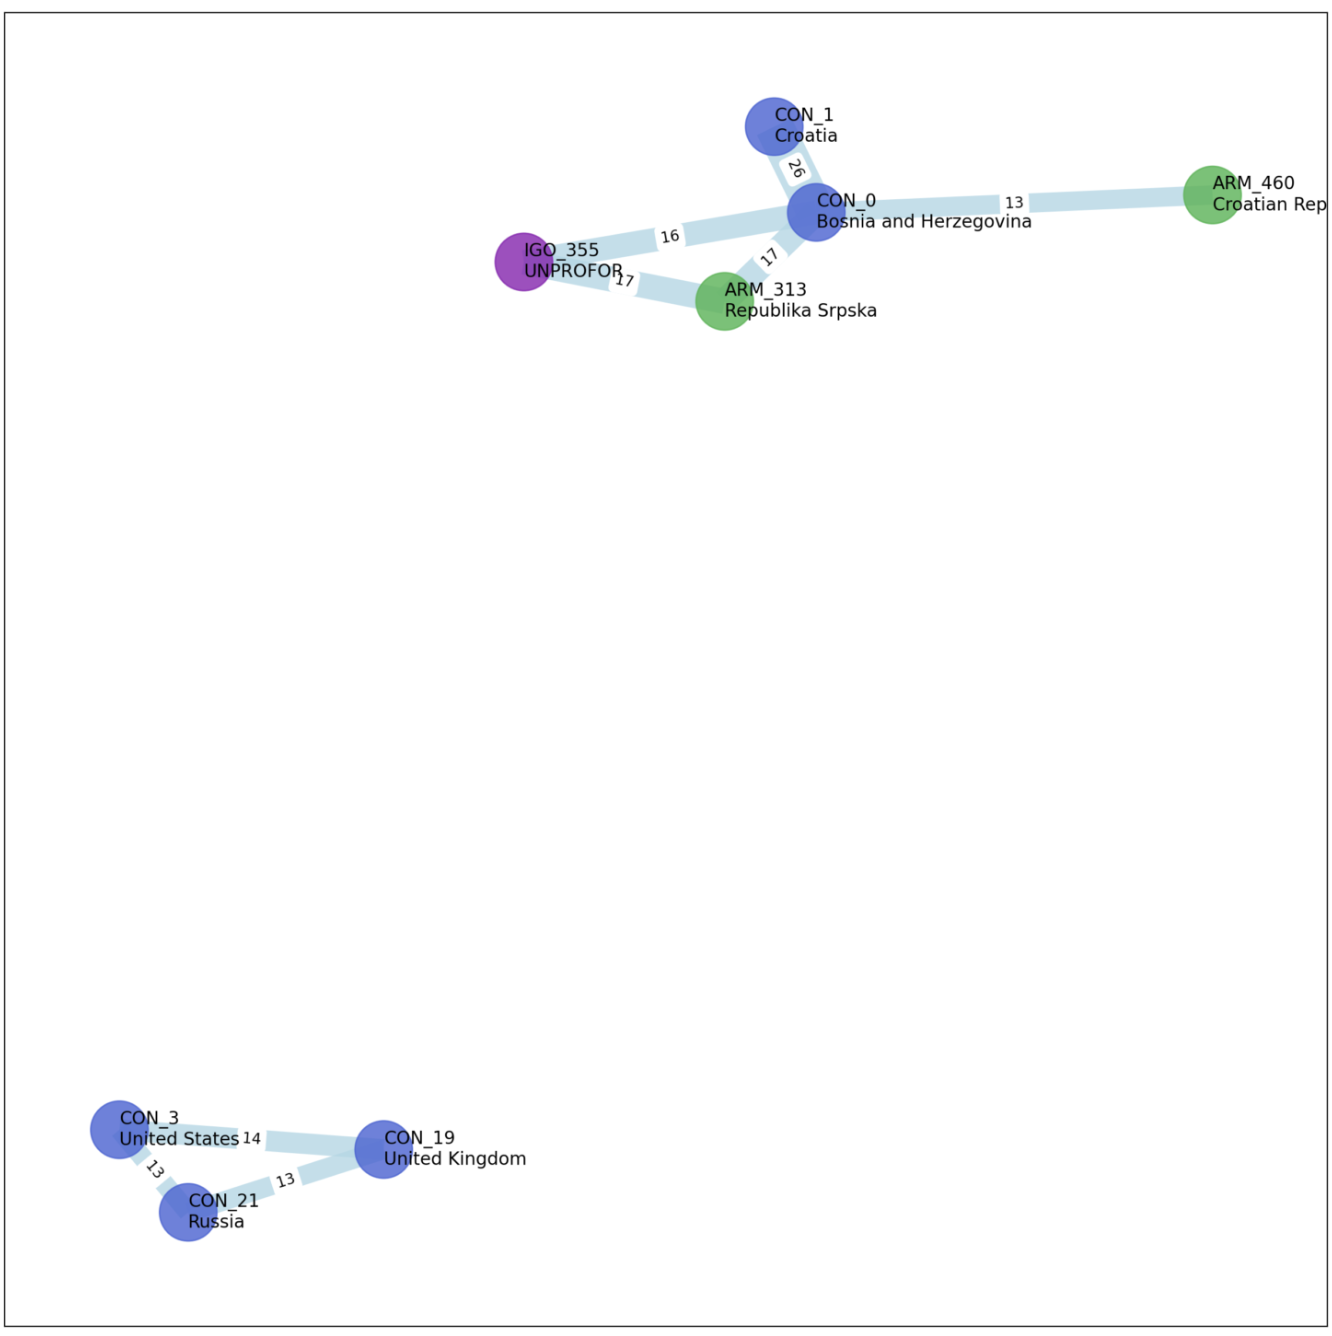
\includegraphics[scale=0.50]{./assets/bosnia_actors.png}
\end{center}
\caption{A graph of the actor co-occurrence matrix from the Bosnia peace process. To qualify for inclusion in the graph a pair of actors must be co-signatories to 13 or more agreements. Two disjoint subgraphs are visible each of which contains a triadic closure. Vertex colour codes for actor type: blue = countries,  purple = IGO, green = armed group.}
\end{figure}

\end{document}
















